% !TeX encoding = UTF-8
% !TeX spellcheck = en_US
% !TeX root = ledgersmb-book.tex

\part{Configuration}
\label{part-configuration}


\chapter{Overview}
\label{cha-configuration-overview}

\section{Introduction}
\label{sec-config-overview-introduction}
This section of the book describes how to set up LedgerSMB and its components.
Configuration \index{configuration} is assumed to be mostly one-off and rather technical in nature.  To find
out which tasks might need to be performed in order to keep the application in good
health the reader is referred to the 'Administration Introduction', \secref{sec-administration-introduction}.

\chapter{Global configuration}
\label{cha-global-configuration}

\section{Apache}
\label{sec-global-config-apache}

Section about installing on \index{apache} Apache 2+

items to be discussed:

\begin{description}
\item [Forwarding of authentication] @@@TODO
\item [PSGI configuration] @@@TODO
\item [performance] cgiD configuration: don't (yet) [but will be supported once all legacy code is gone] @@@TODO
\item [security] suEXEC environment @@@TODO
\end{description}

\subsection{Differences between Apache 1.3 and 2+}
\label{subsec-global-config-apache-13-vs-2}

Explain how to use lsmb with 1.3 instead of 2+.

\section{PostgreSQL}
\label{sec-global-config-postgresql}

\begin{description}
\item [pg\_hba.conf] authentication @@@TODO \index{pg\_hba.conf}
\item [security] local vs IP connections @@@TODO 
\index{Postgres} \index{Postgres Security}
\end{description}


\section{LedgerSMB version numbers}
\label{sec-global-config-ledgersmb-version-numbers}

LedgerSMB version numbers \index{version number} are in the form of Major.Minor.Patch-Optional Tag.
For example, if the production release is \texttt{1.9.27}, then the 1.9 development release is \texttt{1.9.28-dev}.

\begin{description}
\item [Major] An increment in the major release number\index{release number} can mean significant architectural, \gls{API}, functional, or usage changes. It is expected that an upgrade to a new Major version is  going to be planned and tested by the user organization before upgrading.
\item [Minor] An increment in the minor release number may indicate changes to \glspl{API}\index{API}, interfaces, user instructions, etc.  But these changes are not expected to have major impact and should require minor planning and testing. Often small impact enhancements are back-patched to previous Minor versions as patches.
\item [Patch] Increments in the Patch number represent bug fixes, security improvements, or enhancements that do not break existing functionality, usage, or \glspl{API}.  These changes are expected to be applied to an installation as soon as possible.
\item [Optional Tag] Common values include dev, beta, or alpha. Typically, these are only used internally by the LedgerSMB developers.
\end{description}

\section{LedgerSMB Configuration}
\label{sec-global-config-ledgersmb}

LedgerSMB configuration using \texttt{ledgersmb.conf} \index{ledgersmb.conf} is deprecated as of 1 Jan 2023. New functionality may only available when using \texttt{ledgersmb.yaml} \index{ledgersmb.yaml} configuration file.

For the time being there is a conversion step that converts the old 'ledgersmb.conf' to `ledgersmb.yaml`, but the old conf file does not support new functionality.

\subsection{ledgersmb.yaml}
\label{subsec-global-config-ledgersmb-yaml}

For an example of the default, non debug \texttt{ledgersmb.yaml} \index{ledgersmb.yaml} see  \url{https://github.com/ledgersmb/LedgerSMB/blob/master/doc/conf/ledgersmb.yaml}

\subsubsection{\texttt{cookie}}
 @@@TODO

\subsubsection{\texttt{db}}
 @@@TODO

\subsubsection{\texttt{default\_locale}}
@@@TODO

\subsubsection{\texttt{environment\_variables}}
 @@@TODO

\subsubsection{\texttt{extra\_middleware}}
@@@TODO

\subsubsection{\texttt{logging}}
@@@TODO

\subsubsection{\texttt{login\_settings}}
@@@TODO

\subsubsection{\texttt{mail}}

Email \index{mail} can be configured by selecting which of the three available transports to use. The default \texttt{ledgersmb.yaml} file contains examples for the first two.

\begin{description}
    
    \item{\texttt{Email::Sender::Transport::Sendmail}} – Emails are sent using the local server's \texttt{sendmail} \index{sendmail} binary. The configuration parameters are:
    \begin{description}
        \item{\texttt{transport:\$class}} – \texttt{Email::Sender::Transport::Sendmail}
        \item{\texttt{transport:path}} – optionally provide a path to the directory that contains the 'sendmail' binary.
    \end{description}
    
    \item{\texttt{LedgerSMB::Mailer::TransportSMTP}} - Emails \index{email} are sent using a remote SMTP \index{SMTP} server.  The configuration parameters are:
    \begin{description}
        \item{\texttt{transport:\$class}} – \texttt{LedgerSMB::Mailer::TransportSMTP}
        \item {\texttt{transport:host}} – The required host name of the smtp \index{ SMTP} server.
        \item {\texttt{transport:port}} – The required port number of the smtp server. Note this might vary depending on whether TLS or SSL is used.
        \item {\texttt{sasl\_username:\$class}} – The required smtp server authentication method. The values can be `Authen::SASL` or `Authen::SASL::SCRAM`.
        \item {\texttt{sasl\_username:mechanism}} –  The available mechanism are defined at \url{https://metacpan.org/dist/Authen-SASL} or \url{ https://metacpan.org/dist/Authen-SASL-SCRAM} depending on the selected `\$class`.
        \item {\texttt{sasl\_username:callback:user}} – The required SMTP user name.   'the-user' in the default file is a place holder and must be replaced.
        \item {\texttt{sasl\_username:callback:pass}} – The required SMTP password.  'SECURITY-FIRST' in the default file is a place holder and must be replaced.
    \end{description}
    
    \item{\texttt{Email::Sender::Transport::DevNull}} -  Emails are sent to \texttt{/dev/null}, in other words emails are not sent anyplace. This prevents errors in the user interface, but throws away any mail.  There is only one configuration parameter.  This is not a recommended production configuration. It is usually used for testing.
    \begin{description}
        \item{\texttt{transport:\$class}} – \texttt{Email::Sender::Transport::DevNull}
    \end{description}

\end{description}

\subsubsection{\texttt{miscellaneous}}
@@@TODO

\subsubsection{\texttt{output\_formatter}}
@@@TODO  I really don't have a good way to format lists explanations.  See below at \texttt{paths:config:workflows} for an example. Guidance welcome.

\subsubsection{\texttt{paths}}

This section configures the various paths used by LedgerSMB. The configuration parameters are:

\begin{description}
    \item {\texttt{config:locale}} – Path to locale \index{locale path} files. Defaults to \texttt{locale/po}.
    \item {\texttt{config:sql}} – Path to the SQL schema \index{SQL schema path} definition files. 
    \item {\texttt{config:sql\_data}} – Path to the reference and initial SQL database load \index{database load path} files. For example, the names of the countries.
    \item {\texttt{config:templates}} – Path to the templates \index{template path} base directory. Typically set to \texttt{templates}.
    \item {\texttt{config:UI}} – Path to the UI HTML \index{HTML path} files. Defaults to \texttt{./UI/}
    \item {\texttt{config:UI\_cache}} – Path to the location of the UI template cache \index{template cache path}. These are cached after they have been parsed and translated. This improves performance.
    \item {\texttt{config:workflows}} – A list of the Directories where workflow files \index{workflow path} are stored. Contains the default and custom workflows.  Custom workflows are used to override behavior of the default workflows by providing actions, conditions, etc. with the same name and type or by providing workflows of the same type with additional states and actions. Default workflows defaults to \texttt{workflows}. Custom workflows defaults to \texttt{custom\_workflows}. Default workflow path must precede all the custom workflow paths. @@@TODO is the last statement correct?  Can there be more than 2 paths?
\end{description}

\subsubsection{\texttt{printers}}
This section contains a list of printers \index{printing} and their definition.

The default  \texttt{ledgersmb.yaml} file shows two printers \index{printer configuration} named 'Laser' and 'Epson' with the printers defined using the linux \texttt{lpr} command and its arguments. 

This default definition will provide for the selection of the printers named  'Laser' and 'Epson' in the LedgerSMB user interface.

For more information search the internet for 'linux lpr command' or use \texttt{man lpr} at the linux command line.

\subsubsection{\texttt{reconciliation\_importer}}
 @@@TODO

\subsubsection{\texttt{setup\_settings}}
@@@TODO

\subsubsection{\texttt{ui}}
@@@TODO

\subsubsection{\texttt{workflows}}
@@@TODO

\chapter{Per company configuration}
\label{cha-company-config}

\section{Matching your business processes}
\label{sec-company-config-matching-your-business}

By default, LedgerSMB operates such that all optional functionality is available and the user decides to use it or not based on which menu items they select, what fields they enter data into, and what buttons they click.

Removing application roles \index{application roles} (see \appref{app-role-listing}) can limit the visibility of  menu items, data fields, and buttons. This will simplify the users view of the system, reduce training, and better configure LedgerSMB to your business requirements.

Outside of application roles, the only other enforced business process configuration is whether the same person can both create and post transactions. It is called 'separation of duties' \index{separation of duties} and is defined in \secref{subsubsec-company-config-defaults-separation-of-duties}.

LedgerSMB is configured to adjust inventory \index{inventory} when a Sales or Purchase Invoice is posted. This closely matches retail business processes where the customer walks out of the establishment with the product and an invoice \index{invoice} (or receipt).  This functionality can also be used for wholesale shipping applications because LedgerSMB can also produce picking \index{picking} and \index{shipping} shipping documents, just remember that the inventory transaction happens when an invoice is posted.

LedgerSMB uses \gls{FIFO} \index{FIFO} for \gls{COGS} \index{COGS} and inventory calculations.  There are provisions for alternatives, but the code is not yet complete. See \secref{sec-accounting-valuation-inventory} for a detailed explanation of  \gls{FIFO} calculations.

In addition to the above, LedgerSMB has configurable Workflows \index{workflows}. These are not user configurable but your technical support staff should be able to create and edit them. See \charef{part-workflows}.

Contact the \href{https://ledgersmb.org}{development team} for other business process customizations.  In most cases the need for more flexible matching of LedgerSMB to your business processes is understood, but the project has not not yet had any customer requests or development volunteers.

\section{Administrative user}
\label{sec-company-config-admin-user}

@@@ TODO Need to add content explaining the administrative user.

\section{Chart of Accounts}
\label{sec-company-config-coa}

% \chapter{Chart of accounts}
% \label{cha-chart-of-accounts}

The Chart of Accounts or \gls{CoA}\index{Chart of Accounts}\index{CoA} defines how financial reports are organized and summarized.
This section describes the various configuration options available when creating or editing the \gls{CoA}.

\subsection{Predefined Chart of Accounts}
\label{sec-coa-predefined}

LedgerSMB provides predefined Chart of Accounts\index{Chart of Accounts predefined} that can be used out of the box for many businesses.
Most new LedgerSMB setups start with one of the predefined Charts of Accounts and add or delete as necessary to customize it for their business.

There is also an option to import a Chart of Accounts. Importing is described in \secref{subsec-coa-importing}.

The predefined \gls{CoA} files are \gls{XML} format files.

LedgerSMB provides an \gls{XSD} \index{XSD}\index{CoA XSD}file, which might help in developing a custom CoA XML file,  located at \url{https://github.com/ledgersmb/LedgerSMB/blob/master/doc/company-setup/configuration.xsd}.  

To use a custom \gls{CoA} \gls{XML} file, it will need to be placed in the correct directory prior to running \texttt{setup.pl}. The correct directory will be one of the locale sub-directories in \texttt{locale/coa}.

The predefined Chart of Accounts are organized by country and localized. For the United States the following predefined Chart of Accounts are available:
\begin{itemize}
    \item General.xml
    \item GeneralHierarchical.xml
    \item Manufacturing.xml
    \item Service.xml
    \item UCOA-Form990.xml
    \item UCOA-Form990EZ.xml
\end{itemize}

Similar predefined Charts of Accounts are available for other countries and languages.

See \secref{subsec-create-setup-select-coa} for instructions on using these predefined accounts.

The following examples use the \texttt{GeneralHierarchical.xml} account structure.
This file can be found at \url{https://github.com/ledgersmb/LedgerSMB/blob/master/locale/coa/us/GeneralHierarchical.xml}.

\subsection{Account structure}
\label{sec-coa-accounts-structure}

The system allows ordering accounts into groups by assigning accounts to headers. Headers
can themselves be assigned to other headers resulting in hierarchies of account groups.\footnote{Although the
    database structure supports this type of account hierarchy from  1.3, it was not fully in use in reports until  1.4.17. In 1.3 accounts can be assigned a header,
    but headers can't be assigned to headers themselves.}

There are multiple reasons for wanting to use hierarchies. One of those reasons is that expense accounts in prior versions were listed as one long list under Expenses while income accounts are listed as a -usually shorter- list under Income. Personnel expenses are usually spread across multiple expense accounts. With lots of other expense accounts also listed, what's the total expense on personnel?

Another use-case for using hierarchies might be because you're running a "margin business". That is, you're only buying what you're selling and the cost of goods sold is the largest part of your expenses. In cases like this it can be a good idea to use a different setup of the income statement: one where cost of goods sold is immediately subtracted from income, leaving gross margin to cover all other expenses in the company.

In order to set a heading's parent, go to the \menupath{General Journal \ma Chart of Accounts}. Click on the account number. If the account is a heading account that has a parent heading, the resulting screen shown in \figref{fig:config-coa-hierarchy}.

\begin{figure}[H]
    \centering
    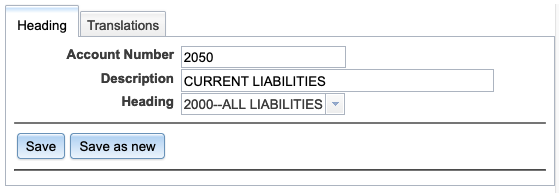
\includegraphics[width=\graphicswidth]{images/gl-coa-heading.png}
    \caption{Configure Account Hierarchy}
    \label{fig:config-coa-hierarchy}
\end{figure}

If the account is a not a heading account, but has a parent heading, then the result is shown in \figref{fig:coa-account-setup}.

\begin{figure}[H]
    \centering
    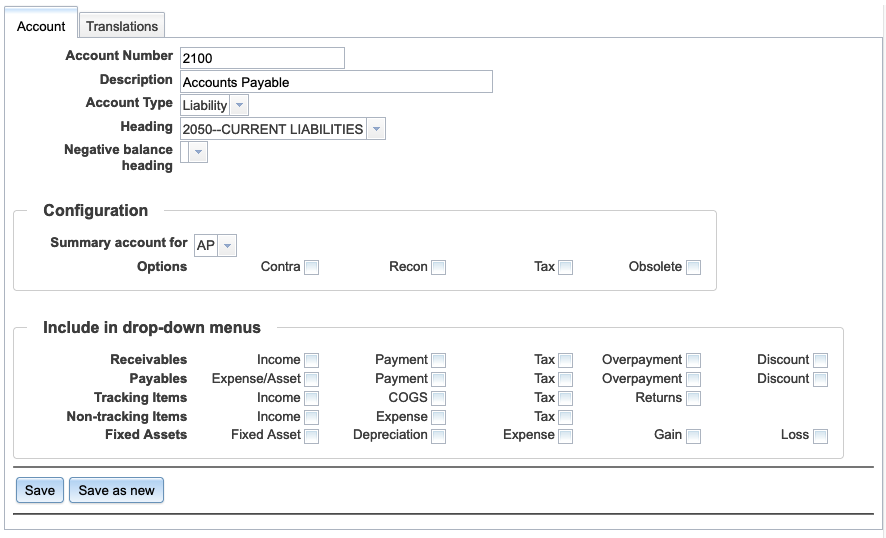
\includegraphics[width=\linewidth]{images/gl-coa.png}
    \caption{Account Setup}
    \label{fig:coa-account-setup}
\end{figure}

If the "Current Earnings" account has been set in \menupath{System \ma Defaults}, see \figref{fig:system-default-accounts}, it is possible to select either the full or non hierarchical (labeled "Account category") account layouts when generating the "Balance Sheet" or "Income Statement" reports.

For example, \menupath{Reports \ma Income Statement} as shown in \figref{fig:config-report-hierarchy}.

\begin{figure}[H]
\centering
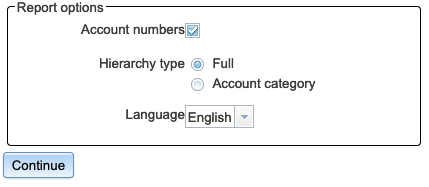
\includegraphics[width=\graphicswidth]{images/reports-select-hierarchy.png}
\caption{Report Using Hierarchy}
\label{fig:config-report-hierarchy}
\end{figure}

\subsection{Account setup}
\label{sec-coa-account-setup}

Headers don't have any configuration, other than their number and description. 

Accounts also
have a number and description, but require additional configuration for the application to work
correctly. 

The settings, which are shown in \figref{fig:coa-account-setup} are described in the following paragraphs.

The main setup consists of the following:

\begin{description}
    \item[Account Number] Income statements and balance sheets reports are ordered by account number. Traditionally, account numbers are 4 digits with accounts being grouped by the first digit, but this type of grouping is not enforced by LedgerSMB. Grouping is handled using headings as explained in \secref{sec-coa-accounts-structure}.
    \item[Description] Should be a relative short, easy to understand description of what the account is used for.
    \item[Account Type] Asset, Liability, Equity, Equity temporary, Income or Expense.
    \item[Heading] Optional entry. Used if this account is a child of a heading account.
    \item[Negative balance heading] Balance sheet account balances should - generally - not be reported as negative amounts\footnote{Notable exception here are "cumulative depreciation" accounts in fixed asset accounting, but these are usually marked as "Contra" -- causing them to be reported as positive numbers..}: a negative asset is in fact a liability. This functionality reports the given account under the primary header as long as the asset/liability is positive and reports it under the "negative balance heading" as soon as the asset/liability turns negative (the expectation is that the alternative header is a liability/asset header instead of an asset/liability header).
\end{description}

\subsubsection{Account configuration}
\label{subsec-coa-account-configuration}

The items in the configuration box as shown in \figref{fig:coa-account-setup} are used to configure the account for use in LedgerSMB.

There are currently three types of optional summary accounts:

\begin{description}
    \item [AR] Marking an account as a summary account for AR means that all outstanding
    receivable amounts will be posted to this account. The Accounts Receivable administration
    will contain the details of which amount is owed by which \gls{customer}.
    \item [AP] Same as the AR account, except for amounts owed to vendors.
    \item [Inventory] This account holds the monetary value equal to the items on stock.
\end{description}

Each account may have zero, one or more of the following options selected.

\begin{description}
    \item[Contra] This checkmark identifies the account as a \gls{contra}\index{contra}account, which means
    that the account is going to hold the opposite of an account it's associated with.
    A good example of this kind would be the depreciation account associated with a fixed
    asset account where the depreciation account contains the credit amount to be added to
    the original asset (debit) value to get the current asset value.
    \item[Recon] This checkmark identifies the account as one which needs reconciliation\index{reconciliation} as
    described in \secref{sec-business-processes-accounting-reconciliation}.
    \item[Tax] This checkmark identifies the account as a Tax (VAT/Sales)\index{tax} account. Tax accounts need

    to be further configured. See \charef{cha-taxes} for further discussion of the
    subject.
    \item[Obsolete] This checkmark identifies the account as not being usable going forward.  The account cannot be deleted because it may
    contain data.
    \label{item:AccountOptionsTax}
\end{description}


\subsubsection{Include in drop-down menus}
\label{subsec-coa-account-links}

In order to enhance the user interface, non-summary accounts may be added to drop down menus throughout LedgerSMB.  Adding
an account is done by checking the box.  Each row in the UI is explained below.

\subsubsection{Receivables checkmarks}
\label{subsubsec-coa-AR-checkmarks}

\begin{description}
    \item[Income (AR\_amount)] This check mark adds the account to the list of accounts
    in the transaction screens which are used to post income on.

    \item[Payment (AR\_paid)] This check mark adds the account to the list of accounts
    to choose from in the Receipts (AR) and Payments (AP) screens as well as the payments lines on invoices and transactions. Additionally, it

    adds the account to the part entry screen as described in \secref{subsec-products-parts-definition}.
    \item[Tax (AR\_tax)] This check mark makes the account show up as a check mark on the
    \gls{customer} (AR) or vendor (AP) entry screen. See \charef{cha-taxes} for further discussion.
    \item[Overpayment (AR\_overpayment)] Adds the account to the receipts screen as discussed
    in \secref{sec-business-processes-payment-processing-overpayments}.
    \item[Discount (AR\_discount)] Adds the account to the customer entry screen's selection
    list for accounts to post payment term discounts on.

\end{description}

\subsubsection{Payables checkmarks}
\label{subsubsec-coa-AP-checkmarks}

The payables UI works the same way as the receivables described in the previous list. The difference is
that the technical names of the configuration identifiers are prefixed by AP\_ instead
of AR\_.

\subsubsection{Tracking Items}
\label{subsubsec-coa-tracking-items}

The items on this line relate to stocked items, i.e. those tracked for inventory: parts and
assemblies.

\begin{description}
    \item[Income (IC\_sale)] Adds the account to the selection list of income accounts on the
    part and assembly definition screens.
    \item[COGS (IC\_cogs)] Adds the account to the selection list of COGS @@@ accounts on the
    part, assembly and overhead definition screen.
    \item[Tax (IC\_taxpart)] Adds a check mark to the part and assembly definition screen
    for the applicable account. See \charef{cha-taxes} for more details on how taxes
    work in LedgerSMB.
    \item[Returns (@@@ Need help here)] @@@
\end{description}

@@@ TODO Labor/Overhead, when part of an assembly, are capitalized in inventory and accounted for in COGS when the resulting assembly is sold. We should add an explanation to that extent somewhere in the book and refer to it from here.

@@@ TODO Labor sold isn't "inventory tracked", so it is a service. Labor/Overhead used to manufacture assemblies is "inventory tracked" and capitalized. We should explain somewhere that Labor sold immediately is a service instead.

\subsubsection{Non-tracking items}
\label{subsubsec-coa-non-tracking-items}

The items on this line relate to untracked (non stocked) items, i.e. services.

\begin{description}
    \item[Income (IC\_income)] Adds the account to the income account selection list in
    the service definition screen.
    \item[Expense (IC\_expense)] Adds the account to the expense account selection list in
    the service definition screen.
    \item[Tax (IC\_taxservice)] Adds a check mark to the service definition screen for the
    applicable account. See \charef{cha-taxes} for more details on how taxes work in LedgerSMB.
\end{description}

\subsubsection{Fixed assets}
\label{subsubsec-coa-fixed-assets}

\begin{description}
    \item[Fixed asset (Fixed\_Asset)] Marks the account as holding the original asset value for the fixed
    assets module, for some classes of fixed assets.
    \item[Depreciation (Asset\_Dep)] Marks the account as holding the cumulative depreciation amount
    for the fixed assets module, for some classes of fixed assets.
    \item[Expense (asset\_expense)] Adds the expense account to the selection list of the fixed assets
    accounting module. See \secref{sec-business-processes-accounting-fixed-asset-accounting} for more details.
    \item[Gain (asset\_gain)] Account to hold book value gain upon disposal of a fixed asset.
    \item[Loss (asset\_loss)] Account to hold book value loss upon disposal of a fixed asset.
\end{description}

\subsection{Special accounts}
\label{subsec-company-config-coa-special-accounts}

Special accounts are set by going to \menupath{System \ma Defaults} and scrolling down to "Default Accounts".

As you can see, in \figref{fig:system-default-accounts} the heading "3999 -- NET MARGIN" has been selected and is the heading which is used as the highest level for the P\&L and lowest level at which income and expenses are being reported in the balance sheet.

\begin{figure}[H]
    \centering
    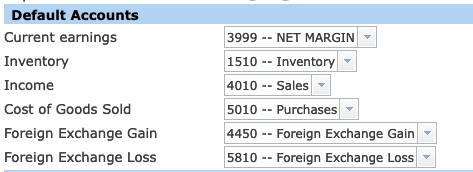
\includegraphics[width=\graphicswidth]{images/system-default-accounts.png}
    \caption{System Default Accounts}
    \label{fig:system-default-accounts}
\end{figure}

The other special accounts are used as follows:

\begin{itemize}
    \item Current earnings - Used to summarize the P\&L result as a single line on the Balance Sheet,
    \item Inventory - Used to summarize the inventory value on the balance sheet.
    \item Income - Used to summarize income on the Income Statement.
    \item Cost of Goods Sold - Used to summarize the cost of goods on the Income Statement.
    \item Foreign Exchange Gain - Accounts for the gain in value differences in foreign currencies when recording payments to invoices in foreign currencies.
    In case an invoice is issued at 1 EUR == 1 USD, but payments arrive when 1 EUR == 0.80 USD, the amount of USD paid is still the invoiced amount, but the EUR amount differs. 
    The EUR difference ends up in the Foreign Exchange\index{foreign exchange} Gain or Foreign Exchange Loss accounts. See \secref{sec-business-processes-payment-processing-fx-payments} for more information.
    \item Foreign Exchange Loss - Accounts for the loss in value differences in foreign currencies when recording payments to invoices in foreign currencies. See \secref{sec-business-processes-payment-processing-fx-payments} for more information.
\end{itemize}

\subsection{Importing chart of accounts}
\label{subsec-coa-importing}

A custom Chart of Accounts \index{Chart of Accounts Import}\index{import Chart of Accounts}can be imported in CSV format by going to \menupath{General Journal \ma Import Chart} and selecting the import file.

The import screen list the required fields. Field content definitions are explained above.

\section{System menu settings}
\label{sec-company-config-system-menu}

This section enumerates the ``System'' menu's immediate children. In some cases the
functionality is too complex and is referred to a chapter of its own.

\subsection{Audit control}
\label{subsec-company-config-audit-control}

\subsubsection{Enforce transaction reversal for all dates}
\label{subsubsec-company-config-audit-control-reversals}


This is a Yes/No value which affects the actions which can be performed on posted financial transactions.
\begin{itemize}
\item No means transactions can be altered or deleted, even after posting them. Note that
if a transaction has been posted before the latest closing date, it can never be altered,
not even when this value is in effect.
\item Yes means transactions can't be altered after posting. This setting is highly preferred and considered the only correct approach to accounting as it assures visible
audit trails and thereby supports fraud detection.
\end{itemize}

\subsubsection{Close books up to}
\label{subsubsec-company-config-audit-control-close-books}


@@@ This item isn't a system setting; shouldn't it move to ``Transaction approval''?? That way system settings (config) and processes are separated.

@@@ My preference is to remove the setting entirely and rely on year-end 
workflow.  We might add an account checkpoint interface as well at some point
--Chris T

It's advisable to regularly close the books after review. This prevents user error changing
reviewed numbers: after closing the books, it's no longer possible to post in the closed
period.

There are also performance benefits to closing the books, because LedgerSMB uses the
fact that the figures are known-stable as a performance optimization when calculating
account balances.

\subsubsection{Activate audit trail}
\label{subsubsec-company-config-audit-control-audit-trail}

This is a Yes/No value which - when Yes - causes the system to install triggers to register
user actions (creation/adjustments/reversals/etc...) executed on financial transactions.


@@@ Once activated, where can we see it the audit trail??

@@@ This setting should go.  In 1.3 the audit trails are always enforced via
triggers so this setting does nothing.  --CT

\subsection{Taxes}
\label{subsec-company-config-taxes}


This page lists all accounts which have the ``Tax'' account option enabled as discussed in \secref{sec-coa-account-setup}.

Each account is listed at least once, but can be listed many times, if it has had different
settings applied over different time periods. E.g. if one of the current VAT rates is 19\%,
today but it used to be 17.5\% until last month, there will be 2 rows for the applicable
VAT account. See \charef{cha-taxes} for further discussion of how taxes work in
LedgerSMB and the choices involved when being required to handle changes in tax rates.

Each row lists the following fields:

\begin{description}
\item [Rate (\%)] The tax rate to be applied when calculating VAT to be posted on this account.
\item [Number] Account number
\item [Valid To] The ending date of the settings in this row. This can apply to the rate as well as the ordering or the tax rules (but usually applies to the rate).
\item [Ordering] This has to do with cumulative taxes.  For example if two taxes
exist and one has an ordering of 0 and one of 1, then the second tax will be
calculated on a basis that includes the first.  One place where this used to be
used was in Quebec, where GST was taxable under PST.
\item [Tax rules] LedgerSMB features a flexible structure to facilitate complex tax
calculations (see \secref{sec-tax-rule-plugins}). By default the ``Simple'' module
is the only one installed.
\end{description}

\subsection{Defaults}
\label{subsec-company-config-defaults}

\subsubsection{Business number}
\label{subsubsec-company-config-defaults-business-number}
   This is used to store an arbitrary identification number for the business.  It
could be used to store a business license number or anything similar.
   
\subsubsection{Weight unit}
\label{subsubsec-company-config-defaults-weight-unit}
   The unit of measurement for weights. @@@ why don't we have a unit of measurement for distance as well??? And maybe a unit of measurement for content?
   
\subsubsection{Separation of duties}
\label{subsubsec-company-config-defaults-separation-of-duties}

% For better or worse this is the spot for the canonical definition of separation of duties.

Separation of duties \index{separation of duties} is a method to help reduce fraud where one employee can't modify the
accounting ledger without another employee's approval.

Select "Yes" if you want to activate separation of duties or "No" if you don't
want to activate it.

In order for separation of duties to be enforced, user roles have to be set differently for each user. This is done by removing the \texttt{draft\_post} role from the users that cannot post and making sure that the users that can post have the role enabled.  See \secref{sec-user-management-authorization} for more details about changing and setting User Roles.

\subsubsection{Default accounts}
\label{subsubsec-company-config-defaults-accounts}

This setting will be used to preselect an account in
the listings of the three categories listed below:
\begin{itemize}
\item Inventory
\item Income
\item Expense
\end{itemize}


\subsubsection{Foreign exchange gain and loss accounts}
\label{subsubsec-company-config-defaults-fx-accounts}

When working with foreign currencies,
the system needs two special purpose accounts. One to post the gains onto which are
caused by foreign currencies increasing in value; the other to post the losses onto
which are caused by foreign currencies decreasing in value.


\subsubsection{Default country}
\label{subsubsec-company-config-defaults-country}

This setting indicates which country needs to be pre-selected
   in country selection lists.


\subsubsection{Default language}
\label{subsubsec-company-config-defaults-language}

The language to be used when no other language has been selected. Several parts of the
application require language selection, such as customer, vendor and employee entry screens.

\subsubsection{Templates directory}
\label{subsubsec-company-config-defaults-templates}

This setting indicates which set of templates - stored in the
   \texttt{templates/} directory - should be used. In a standard installation, the drop down
   lists two items:
\begin{description}
   \item [demo] which contains templates based on \LaTeX, which is more commonly installed but has issues dealing with accented characters
   \end{description}


\subsubsection{List of currencies \& default currency}
\label{subsubsec-company-config-defaults-currencies}

Enter a list of all currencies you want
to use in your company, identified by their 3-letter codes separated by a colon; i.e.
``USD:EUR:CHF''. To ensure correct operation of the application, at least one currency
(the company default currency) must be listed. In case of multiple currencies the first
is used as the company default currency.

\subsubsection{Company data (name /address)}
\label{subsubsec-company-config-defaults-name-address}

The fields ``Company Name'', ``Company Address'',
``Company Phone'' and ``Company Fax'' will be used on printed/e-mailed invoices.

\subsubsection{Password duration}
\label{subsubsec-company-config-defaults-password-duration}

This is an integer value field measuring the validity period in days for passwords set through
the user's \texttt{Preferences} screen. If this field is empty, passwords set through that method
won't expire.

The user has to log into LedgerSMB after this field is changed and prior to the expiration of the previous setting in order for the new duration to take effect.

A user will receive password \index{password duration} expiration reminders upon logging starting a week before password
expiry. When not acted upon, starting two days before expiry an hourly popup will appear
requesting the user to change the password.

The application behaves this way because users with expired passwords won't be able to log in:
their password will need to be reset by a user admin.

\begin{quote}
Note that passwords set by admins for other users expire \index{password expiration} within 24 hours after setting them.
This value is hard coded and can't be overruled. This is a security measure taken to make
sure as few unused accounts as possible exist: Existence of such accounts could open up security
holes.
\end{quote}


\subsubsection{Default E-mail addresses}
\label{subsubsec-company-config-defaults-email}

These addresses will be used to send e-mails \index{email} from the system.
Note that the ``Default Email From'' address should be configured in order to make sure
e-mail doesn't look like it's coming from your webserver. The format to be used is \texttt{``Name'' <e-mail address>} where the e-mail address should be inserted between the
``$\langle$'' and ``$\rangle$''.

\subsubsection{Max per dropdown}
\label{subsubsec-company-config-defaults-max-dropdown}

Some elements in the screens may present a drop down. However, drop downs are
relatively unwieldy to work with when used to present a large number of values
to choose from.

This configuration option sets an upper limit on the number of records to be
presented as drop down.  When the number is exceeded, no drop down is used.  Instead,
a multi-step selection procedure will be used.

\subsubsection{Item numbering}
\label{subsubsec-company-config-defaults-item-numbers}

Many items in the system have sequence numbers: invoices, parts, etc.
These \index{sequence numbers} can be just a number (i.e. 1 or 37) or
they can also be both prefixed and suffixed. For example, INV0001 for invoices and EMP001 for employees or YOU-0001TOO, in which case the next item will be YOU-0002TOO. 

You can only issue every number in the sequence once, but you can issue Y21-001 and Y22-001 by changing the sequence number format at the beginning of the year.

The numbers shown in the input boxes will be used to generate the next number in the
numbering sequence.

\begin{description}
\item [GL Reference number] The default reference number for the next GL transaction.
\item [Sales invoice/ AR Transaction number] This number is used to generate an invoice
number when none is being filled out by the user.
\item [Sales order number ] Same as Sales invoice number, except that it's used for sales orders @@@ layout issue: the label is too big to fit on the page
\item [Vendor invoice/ AP Transaction number] Same as Sales invoice, except that the number
is used for accounts payable transactions. @@@ layout issue: the label is too big to fit on the page 
\item [Sales quotation number] Same as sales order number, except that it's used for quotations.
\item [RFQ number] Request for quotation number is like the sales quotation number, except
that it is used to track which vendors have been asked for quotes.
\item [Part number] All parts, services and assemblies are identified by a unique number.
When an item is created and no number is entered by the user, a number is generated
from this sequence.
\item [Job/project number] Used when creating new projects.
\item [Employee number ] Same as the sales invoice number, used by new employee entry.
\item [Customer number] @@@ is this the control code number? or is this
meta\_number?? -- Meta-number (CT) 
\item [Vendor number] @@@ same question as customer number
\end{description}

\subsubsection{Check prefix}
\label{subsubsec-company-config-defaults-check-prefix}

 The prefix to use when printing checks. There's no check sequence number. That sequence number is requested from the check printing interface, because
checks can be created outside the application as well, meaning the numbers can
get out of sync.

\subsection{Year end}
\label{subsec-company-config-year-end}

@@@ Rename ``Yearend'' in menu interface to ``Year end''.


@@@ IMO this section doesn't belong here, because it's a process, not config, but does it belong in this menu then? IMO it doesn't...


\subsection{Admin users}
\label{subsec-company-config-admin-users}

@@@ Same as Year end; doesn't belong here...

\subsection{Chart of accounts}
\label{subsec-company-config-coa}

@@@ Chart of accounts isn't exactly a ``process'', but it doesn't feel like being pure
config either. At any rate it's a fact that the CoA discussion is a full chapter in and
of itself - so discussion here isn't necessary anymore.

\subsection{Warehouses}
\label{subsec-company-config-warehouses}

Warehouses are stocking locations. They don't have any properties (in the system)
other than that they have a name. Warehouses can be added, modified and deleted from
the \menupath{System \ma Warehouses} menu item.

\subsection{Departments}
\label{subsec-company-config-departments}

Departments can be used to divide a company in smaller pieces. LedgerSMB distinguishes two
types of departments:

\begin{description}
\item [Profit centers] which can be associated with any type of transaction, including AR transactions.
\item [Cost centers] which can be associated with all types of transactions, except AR transactions.
\end{description}

Departments can be created (added), modified or deleted through the \menupath{System \ma Departments} menu item.

\subsection{Type of business}
\label{subsec-company-config-business-types}

Types of business are used in sales operations where customers can be assigned a type
of business. Based on the type of business assignment, quotations, sales orders and
invoices will automatically apply discount rates. For each type of business you enter a description and a discount rate to be applied.

\subsection{Languages}
\label{subsec-company-config-languages}

The language table is the table users can select languages from, both to present
the UI of the application as well as the setting for customers to be used to generate
documents.

This listing should correspond to the actual translations of the application being
available in the program installation directory.

Languages can be added, modified or deleted through the \menupath{System \ma Language} menu item.

\subsection{Standard Industry Code (SIC)}
\label{subsec-company-config-sic}

SI codes feature these three fields:

\begin{description}
\item [Code]
\item [Heading]
\item [Description]
\end{description}

When creating a company you can assign that it an SIC code, irrespective of its role (i.e. customer,
vendor, lead or anything else). An example of an SI code system is the
US's NAICS\footnote{\url{https://www.census.gov/naics/}} code.
Other countries have their own coding systems such
as ANZSIC\footnote{\url{https://www.abs.gov.au/statistics/classifications/australian-and-new-zealand-standard-industrial-classification-anzsic/latest-release}} for Australia and New Zealand
and NACE\footnote{\url{https://ec.europa.eu/competition/mergers/cases/index/nace\_all.html}} for Europe

The SIC field currently doesn't support a specific function in the application and is there
merely for informational purposes. However in the future its role could be extended to include
impact on reports, taxes or other functionalities where type of industry could matter.

\subsection {Templates}
\label{subsec-company-config-templates}

Templates are available to control the output format of many LedgerSMB outputs including Balance Sheet, Sales Orders, etc.

There are 3 types of templates: \LaTeX, HTML, and CSV.
Templates are accessed by navigating to \menupath{System \ma Templates}.
You should see the view shown in \figref{fig:system-templates}.

The template you want to change is selected in the "Template" drop-down. The template format you want to change is selected in the "Format" drop-down.

\begin{figure}[h]
        \centering
        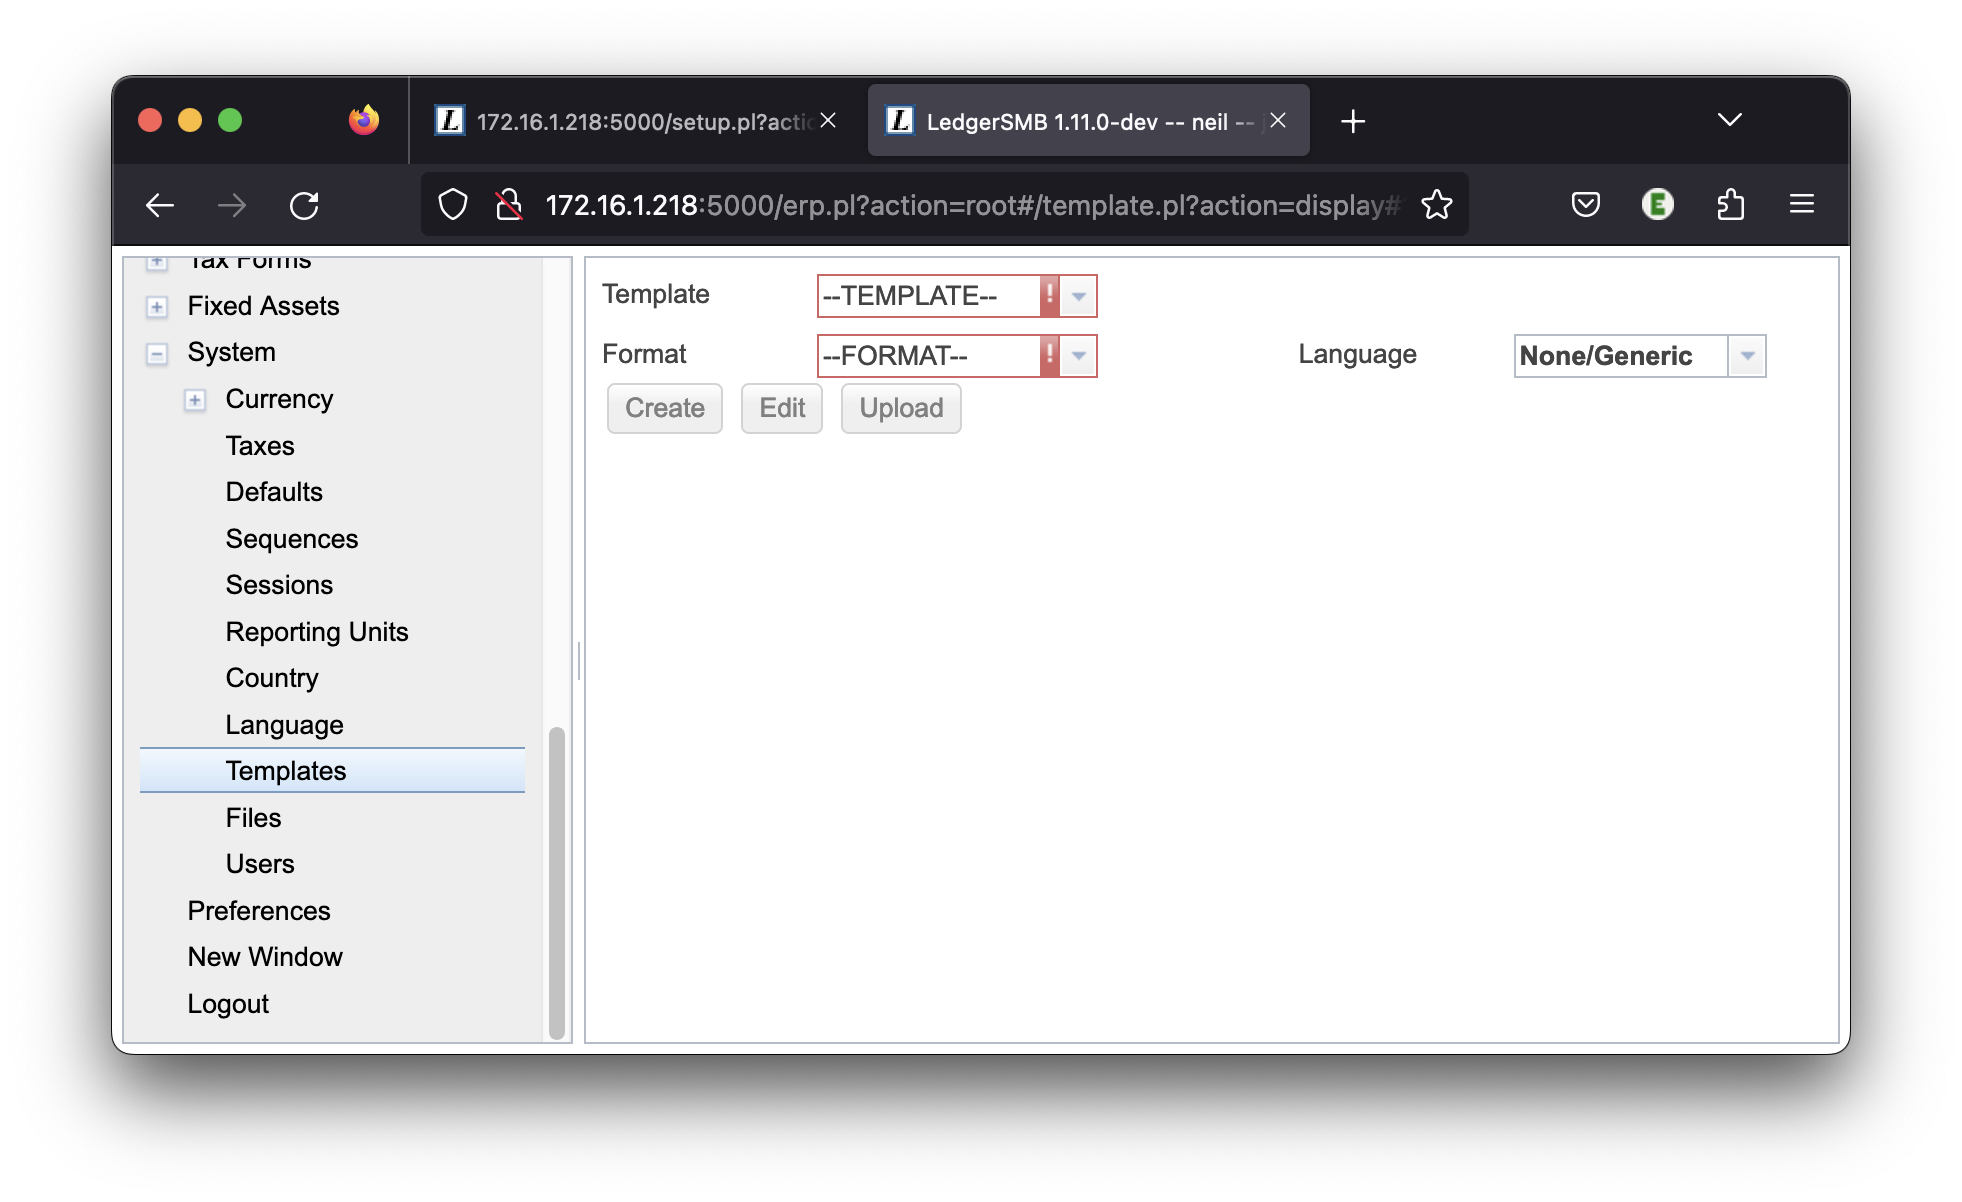
\includegraphics[width=\linewidth]{system-templates.png}
        \caption{System templates screen}
        \label{fig:system-templates}
\end{figure}

\subsubsection{\LaTeX{} templates}
\label{subsec-company-config-latex-templates}

To change a \LaTeX{} template navigate to \menupath{System \ma Templates}.
Select, for example, Template "Invoice" and Format "tex", you should see the view shown in \figref{fig:system-templates-edit-invoice}

\begin{figure}[h]
        \centering
        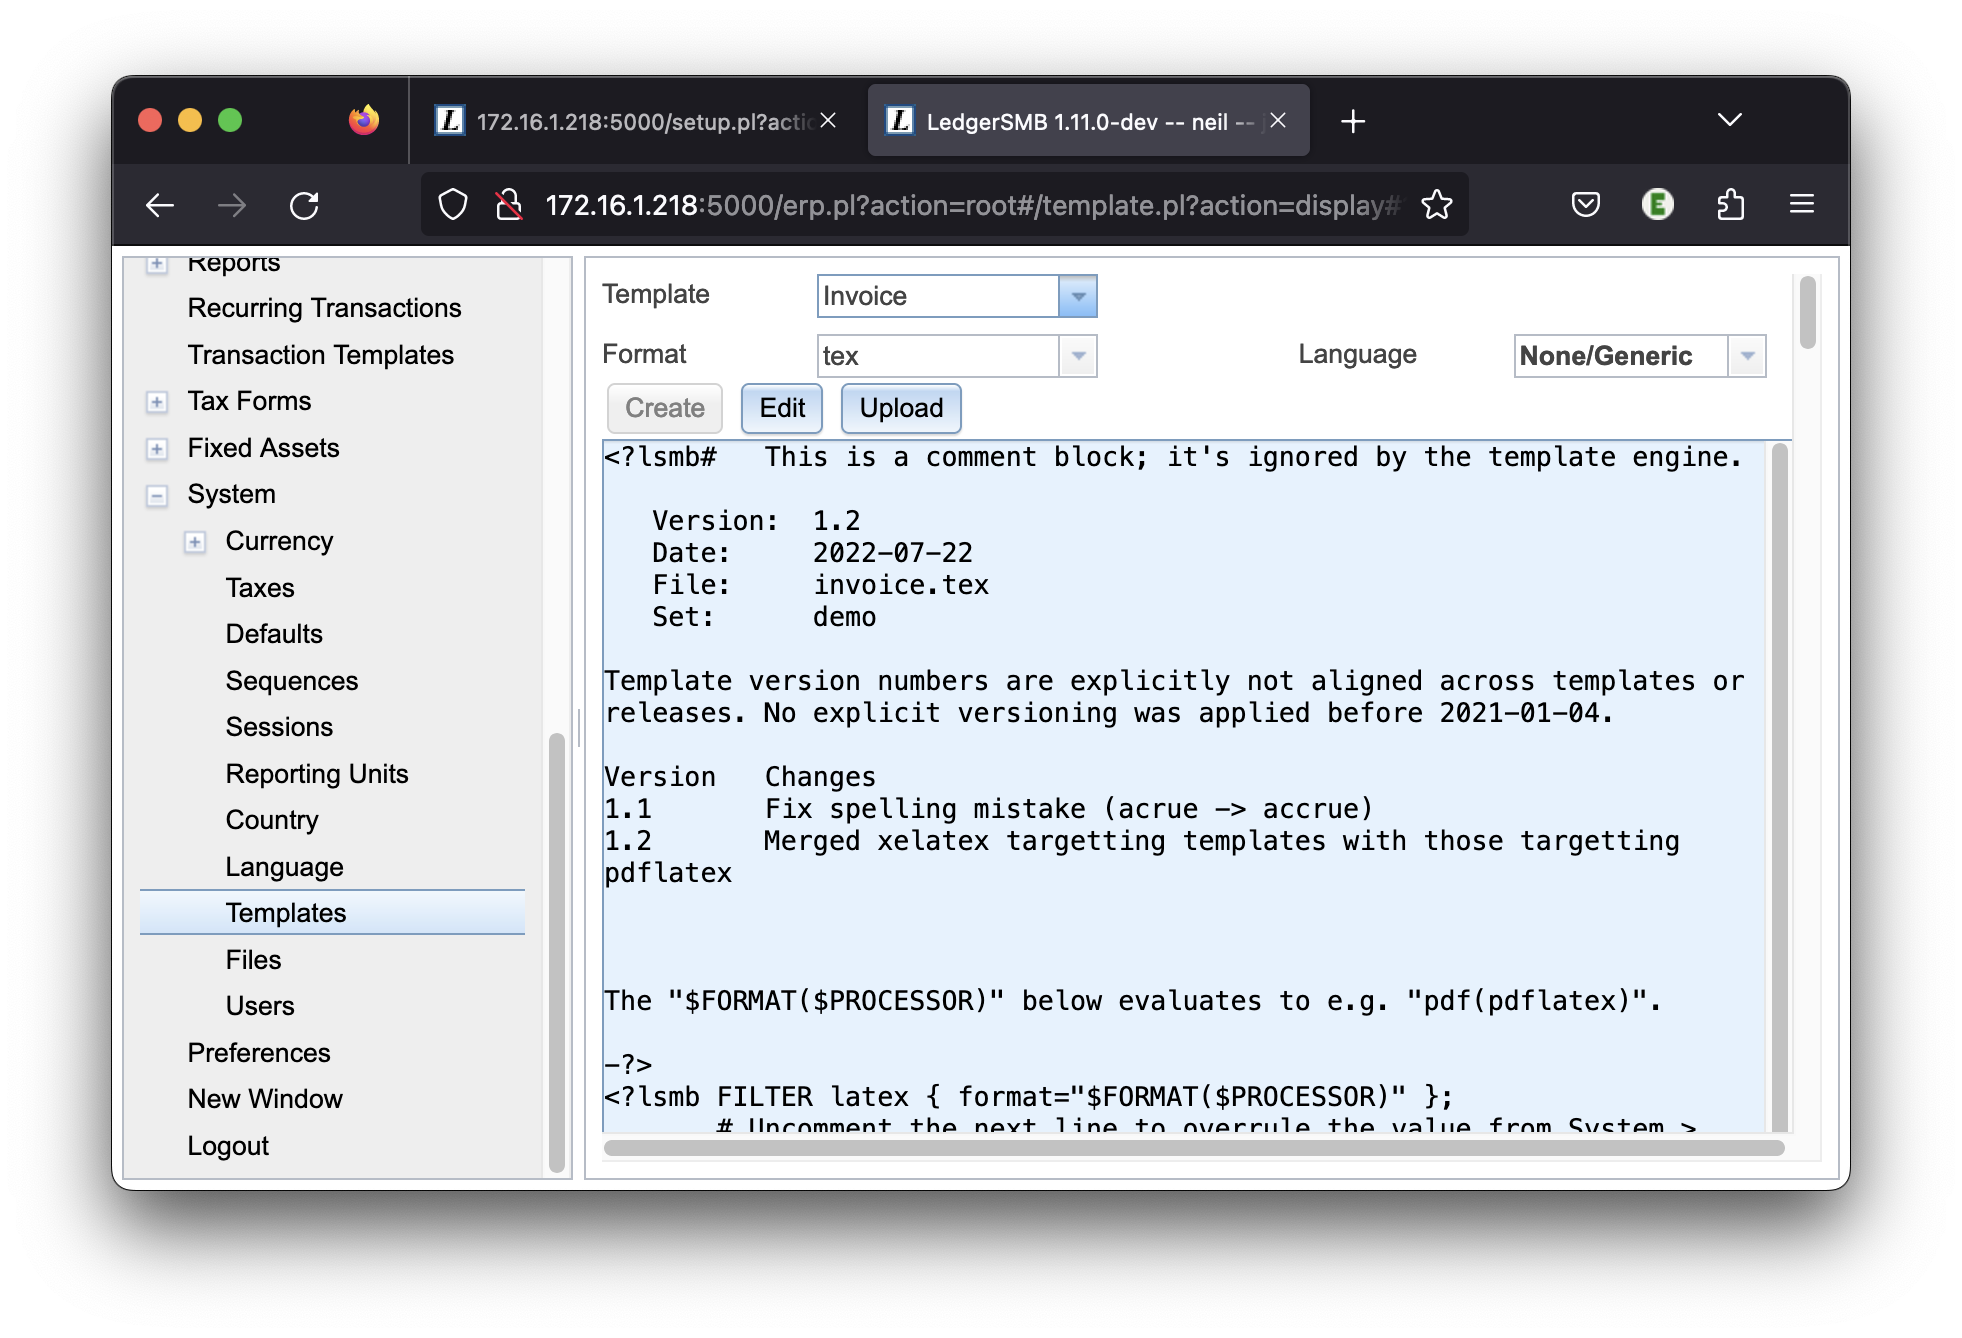
\includegraphics[width=\linewidth]{system-templates-edit-invoice.png}
        \caption{Templates edit invoice screen}
        \label{fig:system-templates-edit-invoice}
\end{figure}

To add a file to the latex template, first upload the image file to the database.  
This can be accomplished by navigating to \menupath{System \ma Files}.

To include this graphic file in your \LaTeX{} document, it needs to be retrieved from
the database and temporarily stored in a location accessible to the PDF
generator. Once the file is in the database, then the function \texttt{dbfile\_path} handles that.

For example, If the graphic file is named "FL\_Logo\_icon\_250x250.png", then add something like the following to the \LaTeX{} template using the \texttt{Edit} button.

\begin{verbatim}
\parbox[b]{.1\textwidth}{%
    \includegraphics[scale=0.7]{%
        <?lsmb dbfile_path("FL_Logo_icon_250x250.png")?>}
}
\end{verbatim}

After editing the template must be uploaded to the database using the \texttt{Upload} button.

\subsubsection{HTML templates}
\label{subsec-company-config-html-templates}

@@@TODO Add HTML specific template info.

\subsubsection{CSV templates}
\label{subsec-company-config-csv-templates}

@@@TODO Add CSV specific template information here.

